\section{Results}
\subsection{Nations Over Time}

\begin{figure}
	\centering
	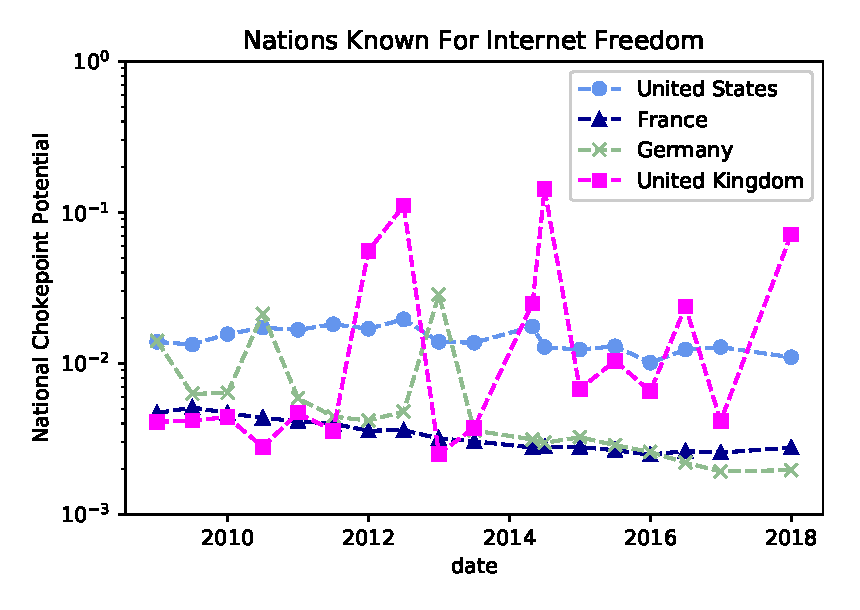
\includegraphics[width=\linewidth]{NodesFree}
	\caption{The number of border ASes required for the US, France, Germany, and Great Britain to intercept 90\% of in-to-out paths over time.}\label{fig:nodesFree}
\end{figure}
\begin{figure}
	\centering
	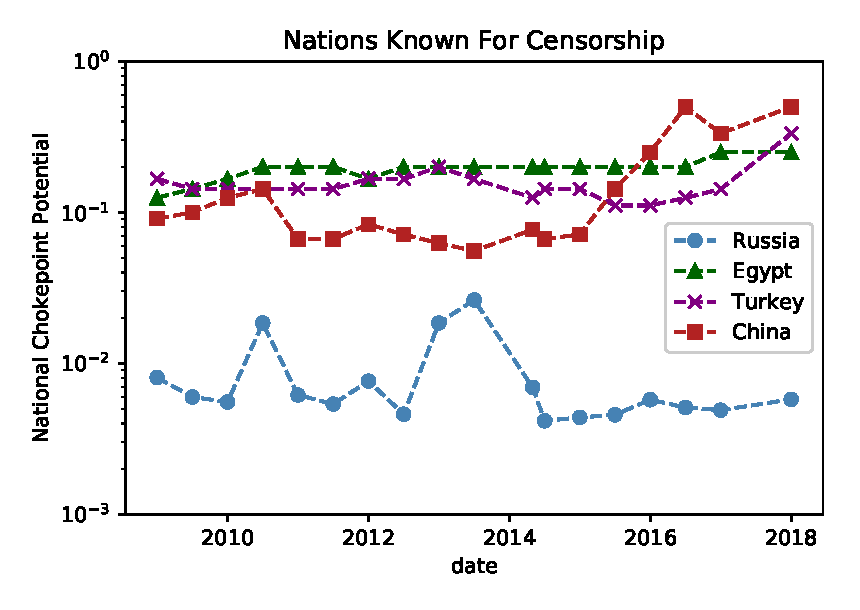
\includegraphics[width=\linewidth]{NodesCensor}
	\caption{The number of border ASes required for Russia, Egypt, Turkey, and China to intercept 90\% of in-to-out paths over time.}\label{fig:nodesCensor}
\end{figure}
\begin{figure*}
	\centering
	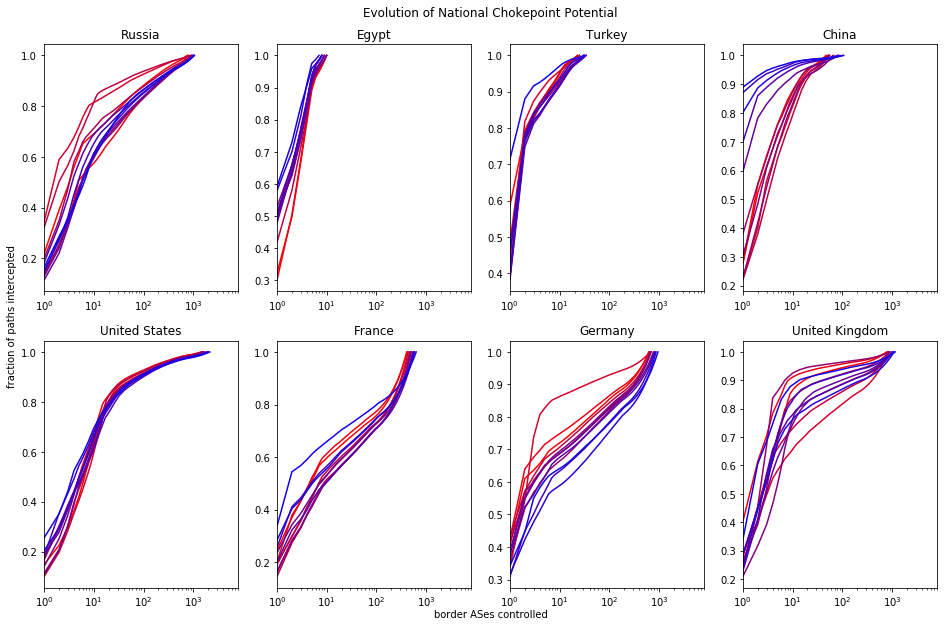
\includegraphics[width=\textwidth]{multi}
	\caption{The capability for various nations to intercept in-to-out paths over multiple years \timerange. Each plot shows for a number of border ASes controlled (x-axis),
	what fraction of in-to-out paths are intercepted (y-axis). Years in blue are more recent, and years in red are further in the past.}\label{fig:multiTime}
\end{figure*}

We have chosen to detail the results of our experiment for 8 nations due to
their histories of censorship practice. First we have chosen 4 nations known to
enact extensive Internet censorship policies. These nations are China, Turkey,
Egypt, and Russia. China has historically been the number one nation in regards
to Internet censorship \cite{censorshipSurvey}. Turkey has recently
dramatically increased its online censorship efforts, by blocking social media
accesses during turmoil and pressuring ISPs to block access to material chosen
by the Turkish government \cite{turkeyCensor}. The Internet of Egypt suffered
severe shutdowns during the Arab Spring of the early 2010s \cite{arabspring}.
The Russian government has passed surveillance laws requiring ISPs to allow the
Russian government access to user statistics \cite{censorshipGeography}. Next
we have chosen the nations of Germany, the United States, France, and the
United Kingdom because, while they have all conducted limited forms of Internet
censorship \cite{censorshipSurvey}, Internet access for these nations is
considered highly open.

To inspect the changes over time for each nation we arrange all the border ASes
belonging to a nation into a list. The list of border ASes is reverse sorted so
that the first AS has the highest chokepoint potential. The sum of all these
chokepoint potentials is 1.0. Then we step through the list, and record the
cumulative chokepoint potential of all the ASes seen so far. If we plot the
number of ASes controled vs the cumulative chokepoint potential for that number
of ASes, we can see how many ASes are required for a certain nation to control
different percentages of paths. We repeat this process for each snapshot to
highlight changes over time.

For instance, consider \figurename \ref{fig:multiTime}.  The x-axis (log-scale,
so that countries with large differences in AS counts can be compared more
easily) for each plot is the number of border ASes controlled, and the y-axis
is the ratio of in-to-out paths intercepted. Each line represents a different
snapshot, with the more red lines being farther in the past and more blue lines
being more recent.

The United States and China are shown here and exhibit some dramatic
differences. First, it is worth pointing out that the United States has many
more ASes than China, hence it's line extends further to the right in these
plots. We also see that China, in all cases, can control a much larger portion
of its paths with much fewer ASes than the United States. This result is
entirely expected. Of more interest is the trends that can be seen over time.
The AS-level topology of China's Internet has evolved such that very few ASes
can intercept nearly all BGP paths. The US has evolved in a different way.
While it has become somewhat easier for the US to intercept most of its paths,
it has become more difficult to intercept around 70\% of its paths and higher.
This suggest an expansion of ASes on the interior and more connections, as well
as a strengthening of the very top ASes.

Not all nations have evolved to a state where it easier to control paths. One
example is Germany, as shown in \figurename \ref{fig:multiTime}. For Germany, a
fairly constant trend shows that it has become more difficult to intercept BGP
paths. Unlike the other examples, any amount of German border ASes intercept
less paths in more recent tests.

In order to compare multiple nations, we have plotted the number of ASes needed
to intercept 90\% of in-to-out paths for each timestamp recorded. These results
are detailed in \figurename \ref{fig:nodesFree} and \figurename
\ref{fig:nodesCensor}.  The distinct behaviors of each nation are rather
striking. We can see a steep decline for some nations known to limit Internet
freedom (China and Turkey) as well as the increase for other nations (Germany
and France). Other nations have stayed more stable. It is worth pointing out
that if a nation has required the same number of border ASes to control many
paths over several years, this suggests that the chokepoints have grown to
intercept more paths. The reason for this is that the number of ASes, and thus
the number of paths, has increased globally over time. This fact makes the
decline in ASes needed for some nations even more glaring.


\subsection{Internet Freedom}

In our test of the relationship between Internet Freedom and national
breakthrough potential, we plotted the Freedom on the Net score of each nation
vs the number of border ASes that that nation needed to in order to intercept
90\% of in-to-out paths. Additionally, we evaluated the relationship with an
Ordinarly Least Squares (OLS) fit, and found that the relationship was
statistically significant, with a p-value $\leq$ 0.002 for 2017. The
relationship held for other timestamps as well. The results for 2017 are shown
in figure \ref{fig:fotn}

\begin{figure}
	\centering
	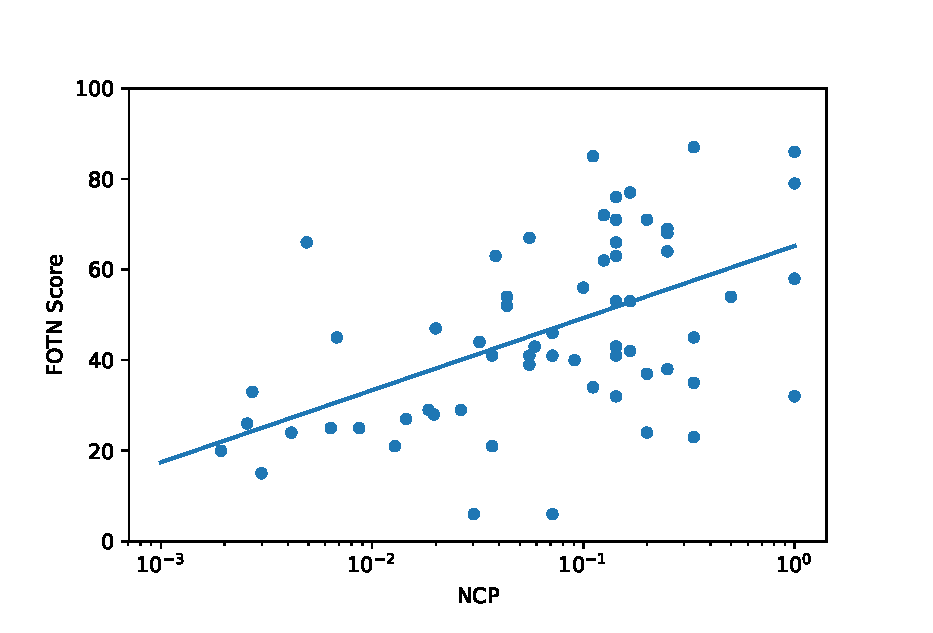
\includegraphics[width=\linewidth]{fotn}
	\caption{The National Breakthrough Potential (in-to-out) for nations plotted against the FOTN score
	of those nations in 2017. A higher FOTN score indicates a less free nation. Our OLS fit is also plotted.}\label{fig:fotn}
\end{figure}

\begin{figure}
	\centering
	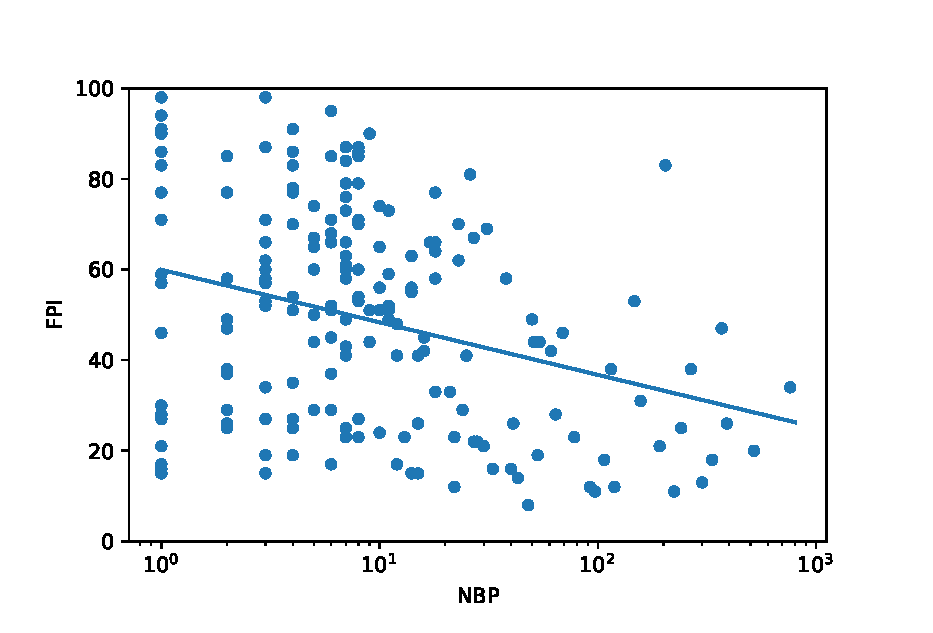
\includegraphics[width=\linewidth]{fotp}
	\caption{The National Breakthrough Potential (in-to-out) for nations plotted against the FPI
	of those nations in 2017. A higher FPI indicates a less free nation. Our OLS fit is also plotted.}\label{fig:fotp}
\end{figure}

For each timestamp we see what appears to be two general modes of behavior.
Nations that are not free or partly free tend to requrie few ASes to intercept
90\% of their paths. Free nations on the otherhand require varying degrees of
large numbers of ASes to control the same portion of their paths. There are
interesting outliers for both situations, however. Countries like Estonia (EE)
or Iceland (IS) are very free but require few border ASes to control most of
their paths. The reason for these outliers is likely that their overall AS
counts are very low. On the other hand, Russia (RU) is a very interesting
outlier in that it is found to be not free by FOTN, but requires a large number
of ASes to control most of its paths. This suggests that the censorship efforts
in Russia might be of types that do not require AS level chokepoints.
